\chapter{Introduction}
In the past electricity production and consumption was localised to small communities. The communities often had one electricity utility company supplying the required energy. As the energy demand increased beyond single production facilities, the solution was to add more production facilities that could support in peak hours. This approach is costly, since such support facilities must be kept in a standby state, ready to deliver additional energy at a moments notice~\citep{RefWorks:46}. As the electric grid expanded, it began to interconnect the communities. The distribution of energy in the grid also became a challenging task. Today's electricity grids are a more global grid that span many communities, and even countries. The consumer plays a passive part in the grid. It is the  operators of the electricity grid that must ensure that energy is delivered at the different consumers, at correct quantities, without overloading the grid. Furthermore must the impact errors and damages have on the grid be minimised~\citep{RefWorks:43}. 

\section{Smart-grid}
In order to combat some of the problems in the grid today, is a new type of electricity grid being deployed. As sensor technology became cheaper and more reliable the electricity utility companies started to integrate sensors in the grid. These sensors delivered information about the performance of key sections of the grid. This information was used to improve the performance of the grid. More types of energy producing devices, such as solar power and wind turbines, got connected to it. This created a need for more control of the grid and the energy production. This laid the foundation for the new grid type called smart-grid~\citep{RefWorks:43}.

The \ab{NIST}[National Institute of Standards and Technology] is tasked with the job of creating and maintaining the standards used for the American smart-grid. The concept behind the smart-grid is to create an electricity grid that enables two way communication. Besides electricity must information about the usage also flow between the consumers and the utility companies. Usage patterns must flow to the engineers tasked with controlling the grid, and control information must flow back to the consumers or control points in the grid. This can ensure the delivery of electricity more efficiently, reliably, and securely ~\citep{RefWorks:42}. 

There are many different kind of stakeholders in today's smart-grid. In order to better understand the needs and relationships between the stakeholders have \ab{NIST} split them in to seven domains. This helps to identify the different user interest in the grid, and their needs.  

\newpage % for nice page formatting 

\begin{figure}[H]
\centering
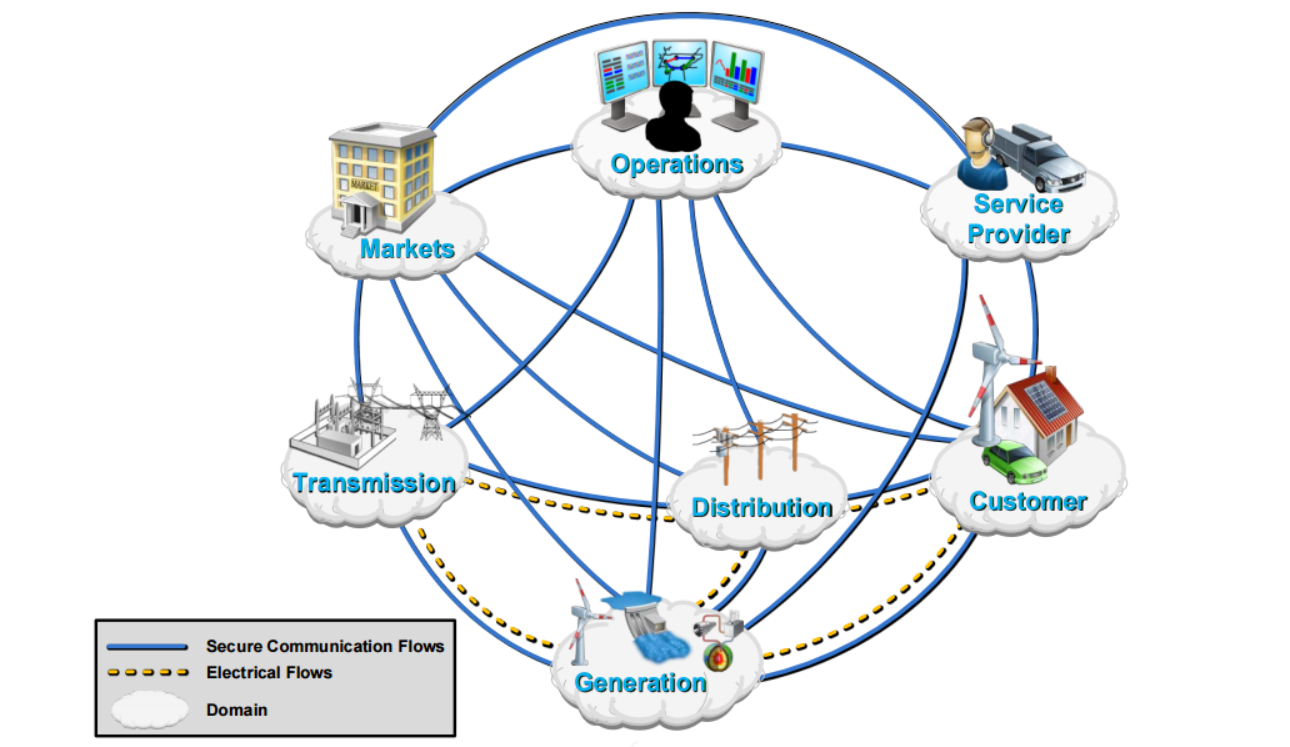
\includegraphics[width=1\textwidth]{billeder/SMARTGRID.png}
\caption[Conceptual model of smart-grid architecture.]{Conceptual model of smart-grid architecture. Source~\citep{RefWorks:41}}
\label{fig:CMOSG}
\end{figure}
 
Figure~\ref{fig:CMOSG} illustrates the seven domains. The seven domains each have a set of functions that is characteristic for the domain~\citep{RefWorks:41}.  
 
\begin{tabularx}{\linewidth}{ r X }
Generation:& The \glsreset{generator}\df{generator} role is the generators of electricity. This is typically coal, oil or nuclear power plants or large-scale hydro generators. This can also include energy storage facilities that stores energy for later distribution. \\\\

Transmission:& \glsreset{transmission}\df{transmission} and transformers that hold the purpose of transporting the electricity over large distances. \\\\

Distribution:& The \glsreset{distribution}\df{distribution} role are the units responsible of electricity distribution to and from the customers. \\\\

Customer:& The \glsreset{customer}\df{customer} role is the consumers of electricity. They may also generate electricity and sell it to the grid. \\\\

Operator:& The \glsreset{operator}\df{operator} role is managers of the movement and production of electricity. They are the group that ensures that the energy is efficiently delivered where it is needed. \\\\

Market:& The \glsreset{markets}\df{markets} is the instance responsible for sale and purchase of electricity between the different instances of the grid. Not just the \df{customer} uses this instance. Utility company can also purchase power from each other to keep up with demand at peek hours. \\\\
\end{tabularx}
\begin{tabularx}{\linewidth}{ r X }
Service Provider:& The \glsreset{service provider}\df{service provider} role are the organisations providing services to the utility companies or the \df{customer}. This could be home automation or information services.  \\
\end{tabularx}

\section{Non-Intrusive Load Monitoring}
The \df{operator} have the responsibility of controlling the flow of energy on the smart-grid. This requires the knowledge of the current consumption and a prediction about the future power requirement. This prediction is generality based on statistical data collected in the grid. If the prediction of the future power requirements can be improved, it is possible to create a better and more efficient power distribution. To accomplish this is a method known as \ab{NILM} developed.

The concept of \ab{NILM} is to use the consumption information collected at household level, and use machine learning techniques to make a qualified guess on what appliances in the household is responsible for the current consumption. By using the information from the active appliances more precise estimates of future consumption can be made. 

In today's smart-grid are all \df{customer}\textit{s} equipped with smart-meters. The smart-meter measures the consumption of the household, and reports it back to the smart-grid. This information can be used by the \df{markets} to automatically create billing information, or by the \df{operator} to regulate the power distribution. Since this information is used for distribution regulation it is send in real-time~\citep{RefWorks:41}. It is this information \ab{NILM} applications hopes to use in order to create better predictions.

\ab{NILM} can also create many opportunities for the \df{service provider}. Using \ab{NILM} it is potentially possible to gesture about the usage of each appliance in a household. This can be used to better inform the resident about power saving opportunities. Studies have shown that detailed information about energy usage, makes the resident use less energy~\citep{RefWorks:33}. Other business opportunities, like selling the statistical information about the usage of specific appliances might also exists.  

\section{The Problem Statement}

This master's thesis seek to investigate some of the common approaches used for \ab{NILM} today, in order to determine the capabilities of such approaches. It is assumed that the \ab{NILM} approaches are used in a modern smart-grid setting. In order to answer this broad question, the following questions must be investigated. 

\begin{itemize}
\item	\textbf{What quality of data can be expected from a smart-meter infrastructure?}\\
In a smart grid is a lot of information collected from various points. For a system that needs the smart-meters data to be collected on a server, what quality can be expected? And where in the infrastructure that collects and transports the information over the Internet, is the quality being compromised? \\
	
	
\item	\textbf{How does sample errors and poor quality affect \ab{NILM} applications?}\\
If the system contains errors, due to samples being lost in the network, how does this impact the \ab{NILM} applications?  Does the quality effect the performance of \ab{NILM} disaggregation? \\
	
\item	\textbf{What behaviours can be detected using \ab{NILM} and where are the limits?} \\
How detailed is it possible to gesture about the behaviour of the appliances in a household? Where are the limits of susses? And what does these limits depend on?  \\
	
\item	\textbf{What can be done to improve the performance of \ab{NILM} technology?}\\
Is it possible to clean data to improve quality and performance? What aspects is the bottlenecks for \ab{NILM} technology today, and how does one improve on this basis? \\

\end{itemize}
If these question is answered it creates a strong foundation for gesturing about the the capability of \ab{NILM}. The main motivation for this study is not to improve grid load predictions, but to get a better basis for validate different \ab{NILM} related business opportunities for \dfs{service provider}.

\section{The Approach}
In order to investigate the questions in the problem statement is real data needed. Research on the  popular methods and definitions in various areas of \ab{NILM}, quality and machine learning has been analysed. The result is used to create the basis of the experiments conducted in this master's thesis. 

\subsection{The Data Approach}
As dataset is the SmartHG dataset used. The SmartHG dataset is a collection of smart-meter data collected from 25 residential households in Denmark. The data is not filtered or cleaned in any way prior usage. This means that the data closely resembles what would be collected in a smart-grid. Furthermore does the dataset contain information about the usage pattern of selected devices. This information can be used to compare inferred usage patterns to the actual. 

\begin{figure}[H]
\centering
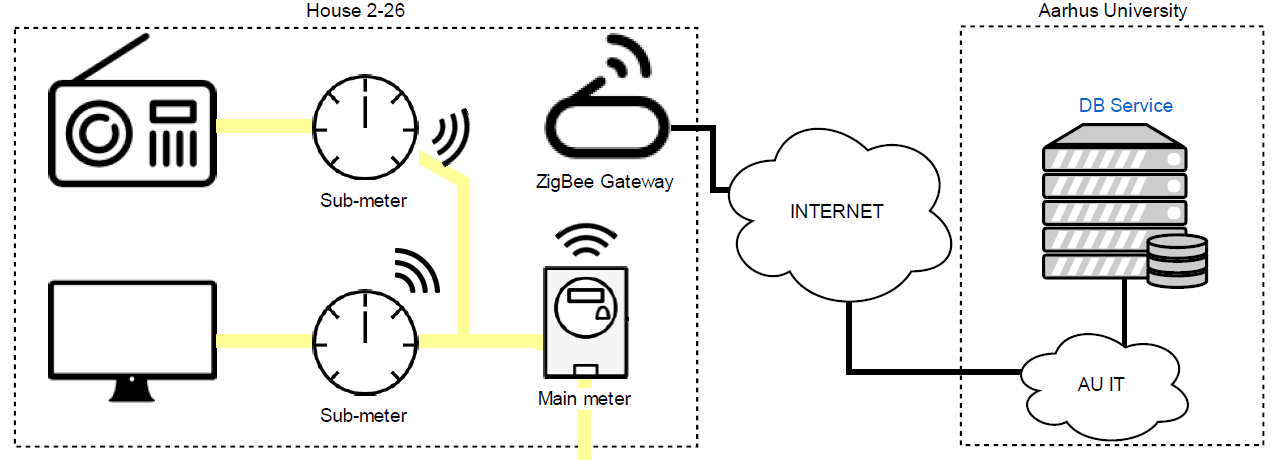
\includegraphics[width=1\textwidth]{billeder/DataCollection.png}
\caption{Data collection process.}
\label{fig:DCP}
\end{figure}
The data is collected from the houses main meter and sub-meters, by attaching a ZigBee module to the meters. The modules transmits the values from the meter to a ZigBee gateway. The gateway transmits the data over the Internet to a database service in the university. This process is illustrated in Figure~\ref{fig:DCP}.

\subsection{The Experiment Approach}
Some of the experiments are conducted on real data, as it would be observed in a real deployment scenario. The behaviours observed in this types of experiment is used to design a series of experiments in controlled conditions, using artificial constructed datasets. These experiments serves the purpose of exposing the properties responsible for the observed behaviour. This improves the understanding of what properties creates wanted and unwanted behaviour. 